The use of cellular broadband for accessing the Internet via tablets and smartphones has increased rapidly as a result of high speed mobile networks such as 3g and 4g. The web browser on these devices are becoming more and more similar in capabilities to their desktop versions. It is possible to run \gls{wrtc} applications in some of them, and these features will become more available with time. This section is going to look at the use of \gls{wrtc} in mobile devices. We start by looking at some of the issues we have to deal with when working with mobile devices, then we will look at performance and quality metrics derived from current research.

\subsection{Performance}
It is feasible to run \gls{wrtc} applications on mobile devices. However, battery consumption,  persistent connectivity, and quality performance remain a big challenge. A lot of work is being done in radio technologies, but the most important factor is how the applications, protocols, and API's are designed\cite{}. First we will look at the characteristics of different mobile networks.

The most used and relevant networks are Wi-Fi, WiMAX, and the different telecommunication networks. Serving wireless video is a significant challenge for already-stressed cellular data networks\cite{erman2011over}. Video traffic requires high bandwidth, imposes latency and packet loss. The key is to deliver video as high in quality as the network supports. By looking at a study testing video and audio quality on two differenet WiMax networks\cite{fund2013performance}, we can see variations of performance in two different locations.
\\
\\
\centerline{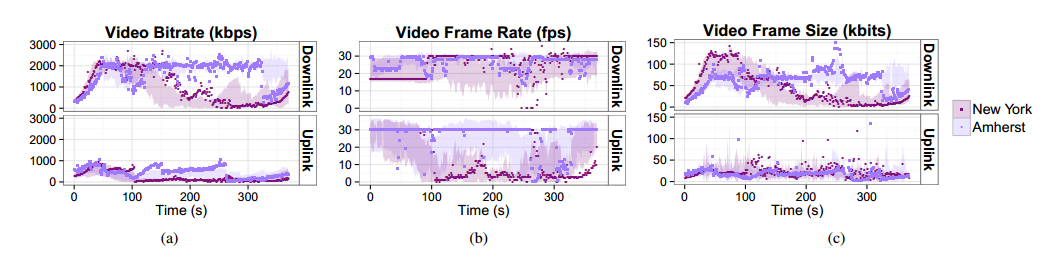
\includegraphics[scale=0.4]{mobile-video-metrics.png}}

\gls{wrtc} adapts to changing link conditions by estimating the available sent bandwidth and passing this estimate to the encoder as a target bitrate. Figure ? show key metrics of video and audio quality for a \gls{wrtc} session sustained over a WiMAX link in two different locations. There is a dramatic difference in performance between the two locations, with the suburban setting always outperforming the urban setting. The uplink(UL) stream has significantly worse video performance, this is probably due to the asymmetry of the celullar link, only 25\% of radio resources are allocated to the uplink. A result of this is a reduced frame rate, this is unfortunate since mobile users are often walking, which makes the video feed have a high motion content.
\\
\\
\centerline{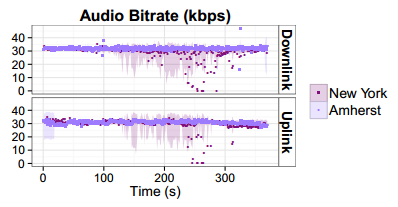
\includegraphics[scale=0.4]{mobile-audio-metrics.png}}

An important thing to mention is that video quality is not that important when it comes to communication, the audio quality is of much more value. We can observe from the firgure 8 that the audio bitrate is mostly consistent, degrading only in extremely poor channel quality.

Another concern is persistent connectivity. For an app to be reachable for incoming connections, it needs some kind of persistant communication channel. Most cellular networks have a firewall preventing incoming TCP connections\cite{isomaki2012considerations}. To keep a TCP connection alive, the applications needs to send some kind of keep-alive packets with a high enough frequency to avoid a connection timeout.
\subsection{Considerations}



\gls{wrtc} has actually handles most of the underlying performance problems that occur in a mobile network as efficiently as possible, but it is important to be aware of these constraints when developing applications. The effect that a mobile users uplink is much worse than its downlink has great impact on a users perception of the connection.